\documentclass[titlepage]{article}
\usepackage{graphicx}
\usepackage{epstopdf}
\usepackage[hmargin=0.5in,vmargin=0.7in]{geometry}
\usepackage{amsmath}
\usepackage{amssymb}
\usepackage{amsthm}
\usepackage{fancyhdr}
\usepackage{tikz-qtree}
\usepackage{datatool}
\usepackage{longtable}
\usepackage[toc,page]{appendix}
\usepackage{url}
\usepackage{listings}
\usepackage{placeins}
\usepackage{hyperref}
%\usepackage[notlot,notlof]{tocbibind}


\def\crv{\cr\noalign{\vskip7pt}} 
\def\a{\alpha } \def\b{\beta } \def\d{\delta } \def\D{\Delta } \def\e{\epsilon }
\def\g{\gamma } \def\G{\Gamma} \def\k{\kappa} \def\l{\lambda } \def\L{\Lambda }
\def\th{\theta } \def\Th{\Theta} \def\r{\rho} \def\o{\omega} \def\O{\Omega}
\def\ve{\varepsilon} 
 \newcommand{\bc}{\begin{center}}
 \newcommand{\ec}{\end{center}}

\numberwithin{equation}{section}

\begin{document}

\lstset{language=Haskell,numbers=left,literate={->}{$\rightarrow$}1 {<-}{$\leftarrow$}1{=>}{$\Rightarrow$}1{(\\}{($\l$}2{*}{$\cdot$}1{>=}{$\geq$}1}

\pagestyle{fancyplain}

\makeatletter
\renewcommand*\env@matrix[1][*\c@MaxMatrixCols c]{%
  \hskip -\arraycolsep
  \let\@ifnextchar\new@ifnextchar
  \array{#1}}
\makeatother

\newcommand{\cond}{\text{cond}}
\newcommand{\emach}{\epsilon_{mach}}
\newcommand{\mbf}{\mathbf}
\newcommand{\w}{\omega}
\newcommand{\hr}{\rule[.5ex]{3.5em}{0.4pt}}
\newcommand{\mytitle}{Airplane Queue Problem}
\newcommand{\myauthor}{Andrey A Popov}

\renewcommand{\sectionmark}[1]{\markright{\thesection\ #1}}
\providecommand*{\lstnumberautorefname}{line} 

\newsavebox{\smlmat}
\savebox{\smlmat}{$\begin{bmatrix}0&1\end{bmatrix}^T$}


\allowdisplaybreaks[1]

\title{\mytitle}
\author{\myauthor}
\date{\today}
\maketitle

\lhead{\fancyplain{}{\rightmark }}
\rhead{\myauthor}
\chead{\mytitle}

\tableofcontents
\listoffigures
\listoftables
\lstlistoflistings
\newpage


\begin{abstract}
In the context of Aircraft queuing, we---using a simulation---optimise for several factors such as customer satisfaction and schedule conformance. 
\end{abstract}

\section{Statement of Problem}
The problem consists of constructing an optimal queuing algorithm for aircraft given an airport and a set of conditions, whilst optimising for several factors including meeting scheduled times, connection times, \&c.

\section{Constructing of simulation}

\subsection{Database Simulation}
The database simulation construction is given in \autoref{lst:dbsim} in the appendix.

Using data obtained from the US Department of Transportation \cite{USDoTData} we try and construct a simulation that conforms as closely as possible to it. 

The simulation calls for there to be 7 different types of aircraft, each capable of carrying 100,150, \&c. up to 400. We then assume that there are  at least 10 people on the flight and that the amount of people is uniformly distributed, as we will factor the amount of people into our calculations thus accuracy in this respect is of little concern.
We assume that each flight lasts exactly one hour and that the connection time has a mean of one hour from the scheduled arrival time and a mean of 15 minutes as seen in \autoref{lst:dbsim_pass} of \autoref{lst:dbsim}. By using the data in \autoref{tab:flightdata} we obtain that the mean departure time of an aircraft is $-4.932468$ minutes, (excluding data that do not have accurate departure statistics) with a mean of $25.5200688$ minutes. A random aircraft is thus obtained as described in \autoref{lst:dbsim_randac} of \autoref{lst:dbsim}.

Using \autoref{lst:dbsim} we get the following sample database:

\DTLloaddb[]{aircraftdb}{aircraftdb.csv}
\begin{table}[h!]
\caption{Sample database of 25 values with passengers omitted due to space constraints}
\label{tab:sampledata}
\centering
\DTLdisplaydb[]{aircraftdb}
\end{table}

\subsection{Airport Simulation}
We then construct the airport simulation, given in \autoref{lst:air}.

We get the following image:
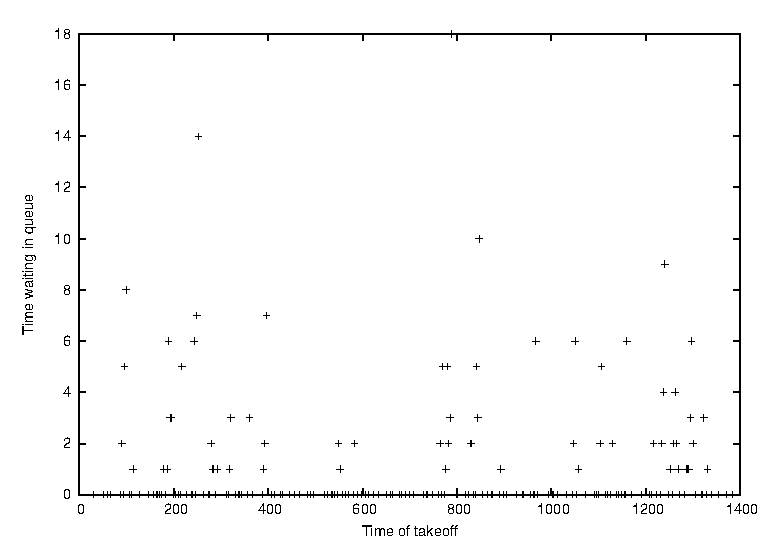
\includegraphics{test.eps}

\newpage
\begin{appendices}
\section{US DoT Data}

\DTLsetseparator{,}
\DTLloaddb[]{USaug2012Ohare}{USaug2012Ohare.csv}

\DTLdisplaylongdb[%
caption={US Department of Transportation US Airways August 2012 Chicago O'Hare Data},%
label={tab:flightdata},%
contcaption={Flight Data (continued)},%
foot={\em Continued overleaf},%
lastfoot={}%
]{USaug2012Ohare}

\newpage
\section{Code}
\lstinputlisting[label={lst:dbsim},caption={dbsimulation.hs},escapeinside={--l@}{@}]{dbsimulation.hs}
\newpage
\lstinputlisting[label={lst:air},caption={air.hs},escapeinside={--l@}{@}]{air.hs}

\end{appendices}

\newpage
\addcontentsline{toc}{section}{References}
\bibliographystyle{plain}
\bibliography{air}

\end{document}